\documentclass[a4paper,10pt]{article}
\usepackage[utf8]{inputenc}
\usepackage[italian]{babel}
\usepackage{hyperref}
\usepackage{graphicx}
\usepackage{wrapfig}
\usepackage{listings}
\usepackage{float}

%opening
\title{IMprovEEsation: Intelligent Musical Evolutionary Entertainment}
\author{Davide Berardi, Matteo Martelli, Marco Melletti, Federico Montori}

\begin{document}

\maketitle

\begin{abstract}

\end{abstract}

\section{Introduzione}

\section{Stato dell'Arte}

\section{Modello del Dominio}
%TODO i componenti alla larga (overview)
\begin{figure}[H]
\centering
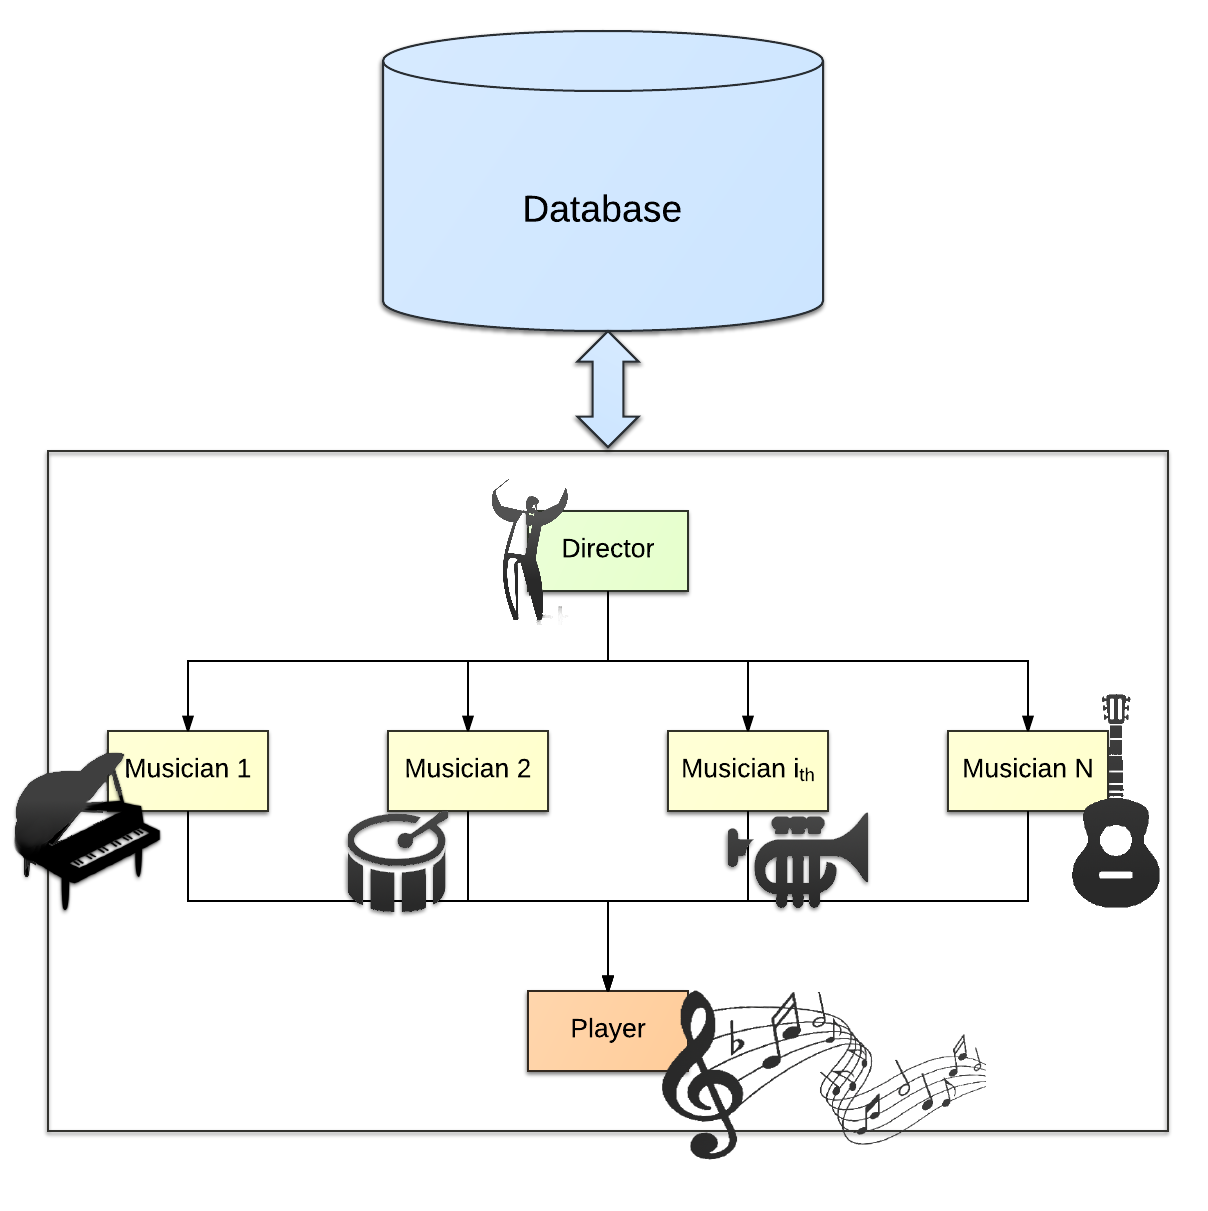
\includegraphics[scale=0.30]{model.png}
\caption{Schema dello scenario di progetto}
\end{figure}

https://www.lucidchart.com/documents/edit/67c03865-48ea-4f6a-b052-e9f9c4cd8196?

\section{Overview dei Componenti}

\section{Interazione e Comunicazione}

\section{Componenti del Sistema}
\subsection{Direttore}

\subsection{Musicista}

\subsection{Player}


\section{Rappresentazione della Conoscenza}
Da qui per le prossime 3 sezioni usiamo i titoli che piacciono tanto 
agli intelligentisti. Pagina 5 del libro di IA. 
Manca interpretazione del linguaggio naturale perchè non sapevo cosa metterci dentro.
\subsection{Regole e Pattern}
\subsection{Database Relazionale}

\section{Ragionamento Automatico}
\subsection{Mente del Direttore}
Come ragiona il direttore quando decide i pattern?
\subsection{Mente del Musicista}
Come ragione il musicista quando decide le note?

\section{Apprendimento}
TODO:blabla generico su come potrebbe apprendere unm musicista basandosi sull'algoritmo genetico:
si fornisce un insieme di samples a cui il musicista cerca di arrivare. 
Alla fine dovrebbe salvare tutto salvare nel database per in modo da non buttare quello appreso.
Per adesso c'è solo l'algoritmo genetico ma spieghiamo comunque come salvaremmo la nuova conoscenza nel DB.  
\subsection{Algoritmo Evoluzionistico}
supercazzola genetica e tante stampe.
\subsection{Sviluppo della Conoscenza}
Spieghiamo qui o in sviluppi futuri? Comnque potremmo proporre nel futuro di salvare nel db 
il risultato del genetico "facendo un match" dei quarter che sono usciti dal genetico con quelli che già
ci sono nel db "aggiustando" le probabilità che già ci sono. Quelle che non ci sono possiamo aggiungerle. 

\section{Risultati Sperimentali}
Dopo tanto sbatto funziona tutto random!

\section{Conclusioni}
Ci vuole un DB supermegagigante!!!

\section{Sviluppi Futuri}

\begin{thebibliography}{50}
  \bibitem{Simpson} Homer J. Simpson. \textsl{Mmmmm...donuts}.
		Evergreen Terrace Printing Co., Springfield, SomewhereUSA, 1998
\end{thebibliography}

\end{document}
